%boost algo
\subsubsection*{Algorithm}
To begin, we performed a simple addition of a value to each of the $rgb$ channels of the hand, such that the average colour of the hand in the processed image is equal to the average colour of the hand in the target image. The algorithm is shown in Equation \ref{eq:boost_algo}.

\begin{equation} \label{eq:boost_algo}
r' = r + \delta_r
\end{equation}

Where 

\begin{equation*}
\delta_r = \mean{r_t} - \mean{r}
\end{equation*}

\nomenclature{$r$}{Value of the red channel of a pixel in the original hand image.}
\nomenclature{$r'$}{Value of the red channel of the pixel after an algorithm is applied.}
\nomenclature{$\mean{r}$}{Average value of the red channel of the original hand image.}
\nomenclature{$\mean{r_t}$}{Average value of the red channel of the target hand image.}
\nomenclature{$g$}{Value of the green channel of a pixel in the original hand image.}
\nomenclature{$b$}{Value of the blue channel of a pixel in the original hand image.}

With the same equation applying for the $g$ and $b$ channels.

\subsubsection*{Results}
In Table \ref{tab:boost_test} we show the results for colour transfers between all possible combinations of our test images.
\begin{longtable}{|N||c|c|c|}
	\caption{Test results of simple addition / subtraction brightening function.\label{tab:boost_test}}\\
	\hline
	\multicolumn{1}{|c||}{No.} & Original & Target & Results \\ 
	\hline
	    \label{row:boost_test_1} &
  \begin{minipage}{.29\textwidth}
    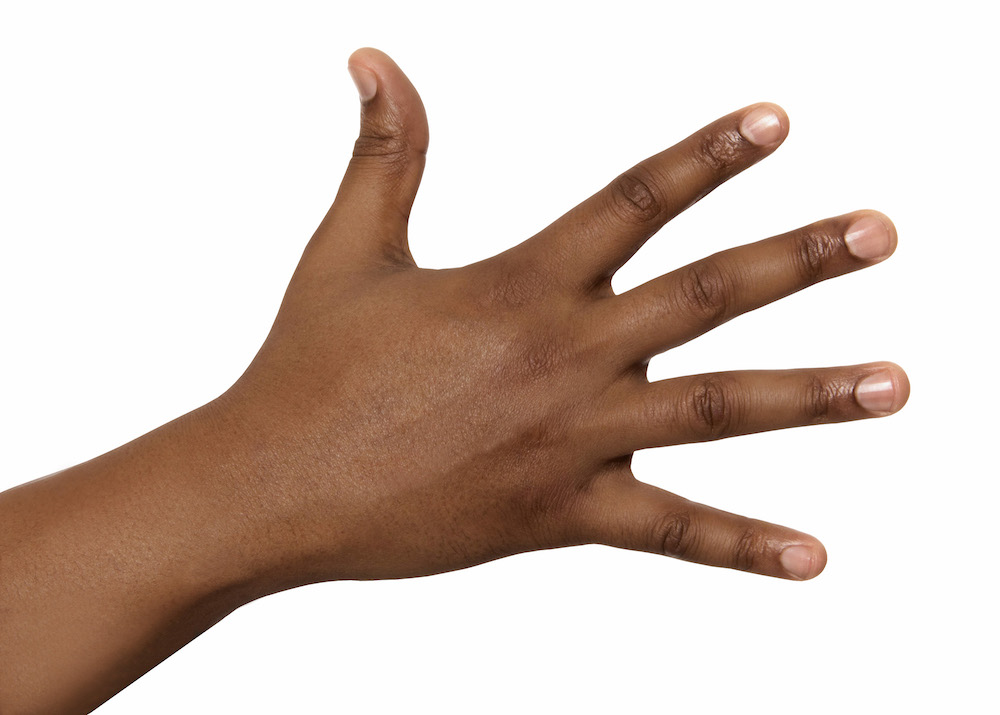
\includegraphics[width=\textwidth,height=\textheight,keepaspectratio]{../inputs/hand_dark.jpg}
  \end{minipage} & 
  \begin{minipage}{.29\textwidth}
    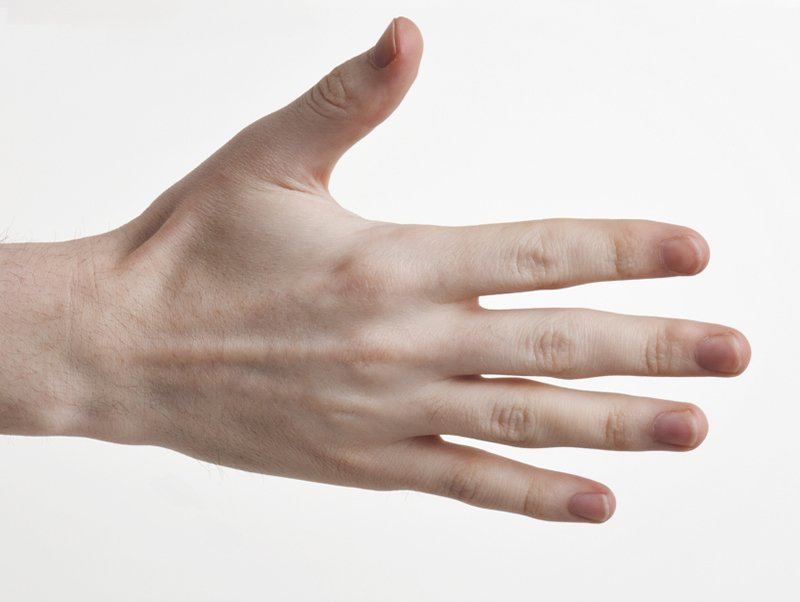
\includegraphics[width=\textwidth,height=\textheight,keepaspectratio]{../inputs/hand_pale.jpg}
  \end{minipage} & 
  \begin{minipage}{.29\textwidth}
    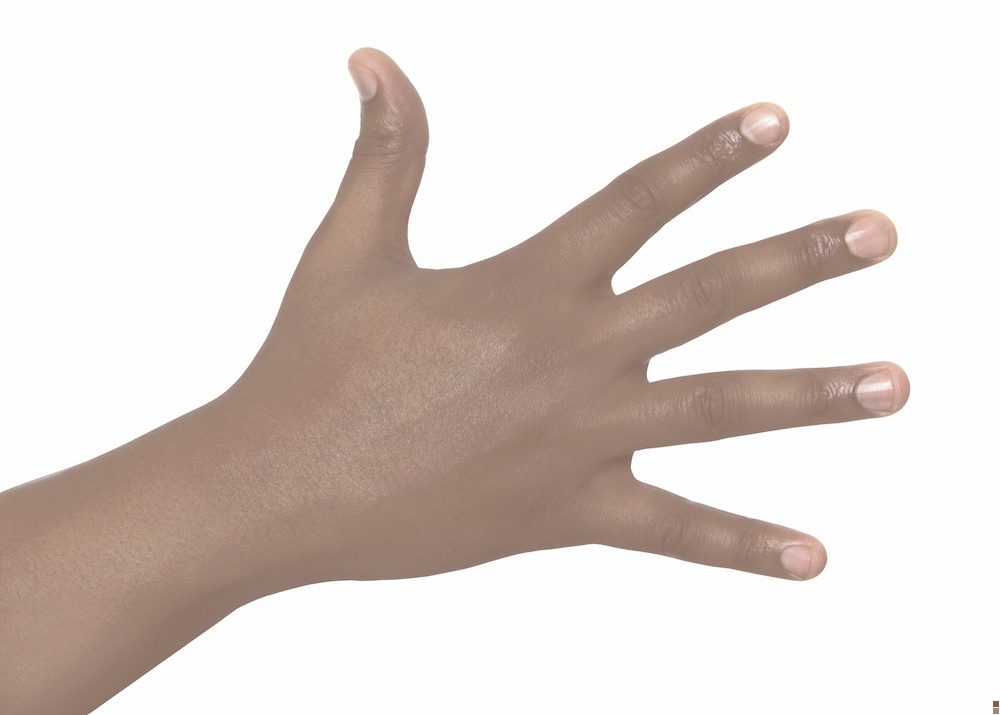
\includegraphics[width=\textwidth,height=\textheight,keepaspectratio]{../rc_test/outputs/debug/hand_dark_to_hand_pale.jpg}
  \end{minipage} \\
\hline
 \end{longtable}

\subsubsection*{Evaluation}
Images of darker skin tones and smaller changes from the original skin tone to the target colour to begin with (Row \ref{row:boost_test_hand_brown_to_hand_dark}) tend to have better results than images with large changes (Rows \ref{row:boost_test_hand_dark_to_hand_light}, \ref{row:boost_test_hand_brown_to_hand_pale}). In the case of changes towards brighter colours, this is because large changes force bright points in the original image to be truncated at white, and also causes dark regions on the image, such as shadows and grooves, to become significantly brighter and less close to true black, giving the image a ``high-key" appearance (Row \ref{row:boost_test_hand_dark_to_hand_light} and \ref{row:boost_test_hand_brown_to_hand_light}).

In addition, we noted that at this stage the transformation from a dark coloured hand to a very pale hand, or even from a mid-toned hand to a pale hand and vice versa is especially unconvincing. (Row \ref{row:boost_test_hand_brown_to_hand_pale}, also see \ref{row:boost_test_hand_dark_to_hand_pale} and \ref{row:boost_test_hand_pale_to_hand_dark})
